\documentclass{article}
\usepackage[document]{ragged2e}
\usepackage{enumitem}
\usepackage{amssymb}
\usepackage[spaces,hyphens]{url}
\usepackage{amsthm}
\usepackage{bbm}
\usepackage{dsfont}
\usepackage{fullpage}
\usepackage{fancyhdr}
\usepackage{titlesec}
\usepackage{hyperref}
\usepackage{url}
\usepackage{xcolor}
\usepackage{stmaryrd}
\usepackage{tikzpagenodes}
\usepackage[T1]{fontenc}
\usepackage[utf8]{inputenc}
\usepackage{CJKutf8}
\usepackage[english]{babel}
\usepackage{titlesec}
\usepackage{pgfplots}
\pgfplotsset{width=10cm,compat=1.9}
\usepgfplotslibrary{external} 
\usepackage{tikz,tkz-tab,amsmath}
\usetikzlibrary{arrows}
\graphicspath{ {./images/} }
\newcommand\E{e}
\newcommand\R{\mathbb{R}}
\newcommand\N{\mathbb{N}}
\newcommand\Z{\mathbb{Z}}
\newcommand\K{\mathbb{K}}
\newcommand\Q{\mathbb{Q}}
\newcommand\C{\mathbb{C}}
\newcommand\T{\mathcal{T}}
\usepackage[headsep=1cm, headheight=1cm]{geometry}
% !TeX spellcheck = en_GB 

\newcommand\dspst{\displaystyle}
\def\prop#1{\underline{\textbf{#1}}}

\def\changemargin#1#2{\list{}{\rightmargin#2\leftmargin#1}\item[]}
\let\endchangemargin=\endlist

%\titleformat{\part}[block]{\filcenter}{}(1em){}
\titleformat{\part}[block]{\Huge\bfseries\filcenter}{\partname{} \\ \thepart}{1em}{\huge}
\renewcommand{\thesubsection}{\Alph{section}.\arabic{subsection}}
\renewcommand{\thesubsubsection}{\Alph{section}.\arabic{subsection}.\arabic{subsubsection}}

%Defines emphasis color
\definecolor{rycolor}{RGB}{200,20,255}
\definecolor{note}{RGB}{100,100,100}

%Defining a multi-line comment
\newcommand{\comment}[1]{}

\title{Programming and Algorithms Project \\ Annex - Julia and Fatou sets}

\author{Christopher Mazzerbo}
\date{Last updated on \today}


\begin{document}
\setcounter{section}{1}

\titlespacing{\subsubsection}{5mm}{0cm}{0cm}

%title

\fancypagestyle{plain}{
\fancyfoot{}
}
\pagestyle{plain}
\maketitle
\vspace{5mm}
\hrule
\pagebreak


%Edit header
\pagestyle{fancy}
\fancyhf{}
\fancyhfoffset[L]{1cm} % left extra length
\fancyhfoffset[R]{1cm} % right extra length
\rhead{Programming and Algorithms Project - fractal art}
\lhead{\bfseries Christopher Mazzerbo}
\fancyfoot{}
\fancyfoot[C]{\thepage}

\tableofcontents
\pagebreak



In this document we will use the notation $\overline{\C}$ to denote the Riemann sphere : $\overline{\C} = \C \cup \lbrace \infty \rbrace$. \\

\subsection{Definitions}

\prop{Meromorphic function} : \\
\begin{changemargin}{1cm}{0cm}
Let $f : \overline{\C} \to \overline{\C}$. We say $f$ is \textit{meromorphic} on an open set $D \subset \overline{\C}$ if $f$ is holomorphic (that is to say, complex-differentiable) on $D \backslash S$ where $S$ is a set of isolated points ($\#S < \infty$). \\
\vspace{2mm}
I will write $M(X)$ the space of all complex functions that are meromorphic on $X \subseteq \overline{\C}$.
\end{changemargin}
\vspace{5mm}


\prop{Julia sets, Fatou sets} : \\
\begin{changemargin}{1cm}{0cm}
Let $U$ be an open subset of $\overline{\C}$ and let $f : U \to \overline{\C}$ be a meromorphic function. \\
$$\mathcal{F}_f = \biggr\lbrace z \in U, \, \, \exists V_z \subset U, \, \, \exists (f^{n_k})_{n_k \in \N}, n_1 < n_2 < \dots, \quad (f^{n_k}) \text{ converges uniformly on compacts subsets of } V_z \biggr\rbrace$$
Taking $U = \C$ yields what we call the \underline{Fatou set} of $f$, and we call the complement of this set, the \underline{Julia set} \cite{Sut14} section 5. We then have $\C = \mathcal{F}_f \oplus \mathcal{J}_f$. \\
\vspace{2mm}
It's important to know that $M(\overline{\C}) \ni f \mapsto \mathcal{J}_f \in \text{Julia sets of }M(\overline{\C})$ is not a bijection. \\
Two \textit{different} functions can have the same Julia set \cite{Lev97}.
\end{changemargin}
\vspace{5mm}
\pagebreak

\subsection{Two examples}

\subsubsection{Example of $w \in \mathcal{J}_f$ for a very simple $f$}

Consider $f : z \mapsto z^2$, and $w = 1$. \\
\vspace{5mm}
We will prove $w \in \mathcal{J}_f$ by finding a sequence $(z_k)_k$ for which iterates of $f$ around any neighbourhood $U$ of $w$ do not have any uniformly converging subsequences on any compact subset of said neighbourhood. \\
\vspace{5mm}
\begin{proof}
Consider $r > 0$, defining a neighbourhood $U$ of $w$ by $U = B(w,3r)$. \\
\vspace{2mm}

Let's take a sequence $(z_k)_{k \in \N}$ defined by $z_k = w - \frac{r}{k}$. It's easy to see $z_k$ converges to $w$. \\
\vspace{5mm}
Now consider $f^n(z_k)$ for a fixed $k$. \\
We can deduce from basic power properties that : \\
$$f^n(z_k) \underset{n \to \infty}{\longrightarrow} 0$$
However : \\
$$f^n(w) \underset{n \to \infty}{\longrightarrow} 1 \text{ because } f^n(w) = f^n(1) = 1 \text{ for all } n$$
But then we have $\lVert f^n(z_k) - f^n(w) \rVert \underset{n \to \infty}{\longrightarrow} 1$ for all $k$, which contradicts uniform convergence of $f^n$ or any of its subsequences. \\
This result is true without having to bring up compactness as the discontinuity of $f^n$'s limit in this neighbourhood is independent of the subset we're studying. \\
\vspace{2mm}
Therefore, $w = 1$ is \textbf{not} in the Fatou set. \\
\vspace{5mm}
We know that $\overline{\C} = \mathcal{F}_f \oplus \mathcal{J}_f$, so $w \notin \mathcal{F}_f \Rightarrow w \in \mathcal{J}_f$. 
\end{proof}

\subsubsection{Example of an interesting $w \in \mathcal{F}_f$}

In this example, subsequences of the iterates are required, to illustrate the necessity of this argument in $\mathcal{J}_f$'s definition. \\
\vspace{5mm}

Consider $f(z) = z^2-1$. \\
\vspace{2mm}
Now take $w = -1$. \\
\vspace{2mm}
We will prove $w \in \mathcal{F}_f$ by choosing a neighbourhood of $w$ in which all sequences have a convergent subsequence on compact subsets of itself. \\
\vspace{5mm}

\begin{proof}

We will consider the ball $\overline{B(w,\varepsilon)}$ for $0 < \varepsilon < \frac{1}{5}$. \\
A maximal $\varepsilon$ satisfying this proof can be found \textcolor{blue}{\underline{\href{https://www.wolframalpha.com/input?i=positive+solution+of+\%CE\%B5+\%3D+\%282\%CE\%B5\%2B\%CE\%B5\%5E2\%29\%5E2}{here}}}. \\
\vspace{5mm}

$$\forall z_0 \in \overline{B(w,\varepsilon)}, \qquad z_0 = w+k_0e^{i \theta_0} \quad 0 \leq k_0 \leq \varepsilon, \quad \theta_0 \in [0, 2 \pi[$$
and : \\
\vspace{-3mm}
\begin{align*}
z_1 = f(z_0) &= z_0^2-1 \\
&= (w+k_0 e^{i \theta_0})^2-1 \\
&= 1 - 2k_0e^{i \theta_0} + k_0^2 e^{2i \theta_0}-1 \\
&= -2k_0 \underbrace{\left( e^{i \theta_0}- \frac{k_0}{2} e^{2i \theta_0} \right)}_{\text{modulus } \leq 1+ \frac{k_0}{2} }
\end{align*}
\vspace{-2mm}
It's then easy to see that $f(z_0) \in \overline{B(0,2 \varepsilon + \varepsilon^2)}$. \\
\vspace{5mm}

From $z_1 \in \overline{B(0, 2\varepsilon)}$, as $\varepsilon < \frac{1}{5}$ we have $\lvert z_1 \rvert < \frac{2}{5} + \frac{1}{25} = \frac{11}{25}$. \\
Reusing the notation from earlier, we have $z_1 = 0 + k_1 e^{i \theta_1}$ for $0 \leq k_1 \leq 2\varepsilon + \varepsilon^2$ and $\theta_1 \in [0,2 \pi[$. \\
$$f(z_1) = \underbrace{k_1^2}_{\leq \frac{121}{625} < \frac{125}{625} = \frac{1}{5}}e^{2i \theta_1}-1$$
Which finally implies $f(z_1) \in \overline{B(w,\varepsilon)}$ again. \\
\vspace{5mm}

We have found a neighbourhood $B(w,\varepsilon)$ of $w$ in which any sequence of iterates has terms in one of or both of the sets $\overline{B(w, \varepsilon)}$ and $\overline{B(0, 2 \varepsilon)}$. \\
\vspace{2mm}
$\overline{B(w, \varepsilon)}$ is a the (compact) closure of the neighbourhood, so the Bolzano-Weierstrass theorem guarantees that we can take a subsequence of iterates (specifically such that we exclude all terms in $\overline{B(0, 2 \varepsilon)}$) which will converge (sequential compactness) in $\overline{B(w, \varepsilon)}$. \\
\vspace{5mm}

Thus we conclude $w \in \mathcal{F}_f$. 
\end{proof}

Note that this proof \textit{requires} the definition to extend to subsequences, because of how the given sequences of iterates of $f$ have values in disjoint sets. \\
\vspace{2mm}

Here is a visual representation of this disjointness (made interactive \textcolor{blue}{\underline{\href{https://www.geogebra.org/m/eee6ukbk}{here}}}) : \\
\vspace{-3mm}
\begin{center}
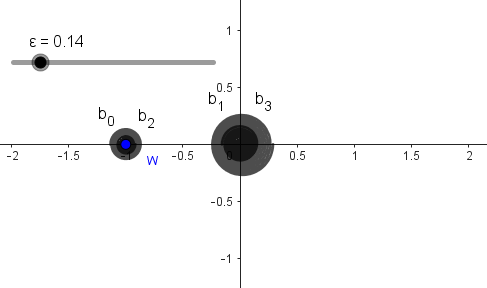
\includegraphics[scale=0.9]{complementminus1} \\
\textit{Fig. 1 - First terms of a sequence of sets $(b_n)$ where $b_n = f^n(B(w, \varepsilon))$}
\end{center}

As goes the proof, the maximal possible $\varepsilon$ for which the proof is valid is actually slightly greater than $\frac{1}{5}$ and can be obtained by solving $\varepsilon = (2 \varepsilon + \varepsilon^2)^2$ for $\varepsilon > 0$. Here is an image showing how this $\varepsilon$ appears in the Fatou component $w$ is in : \\
\begin{center}
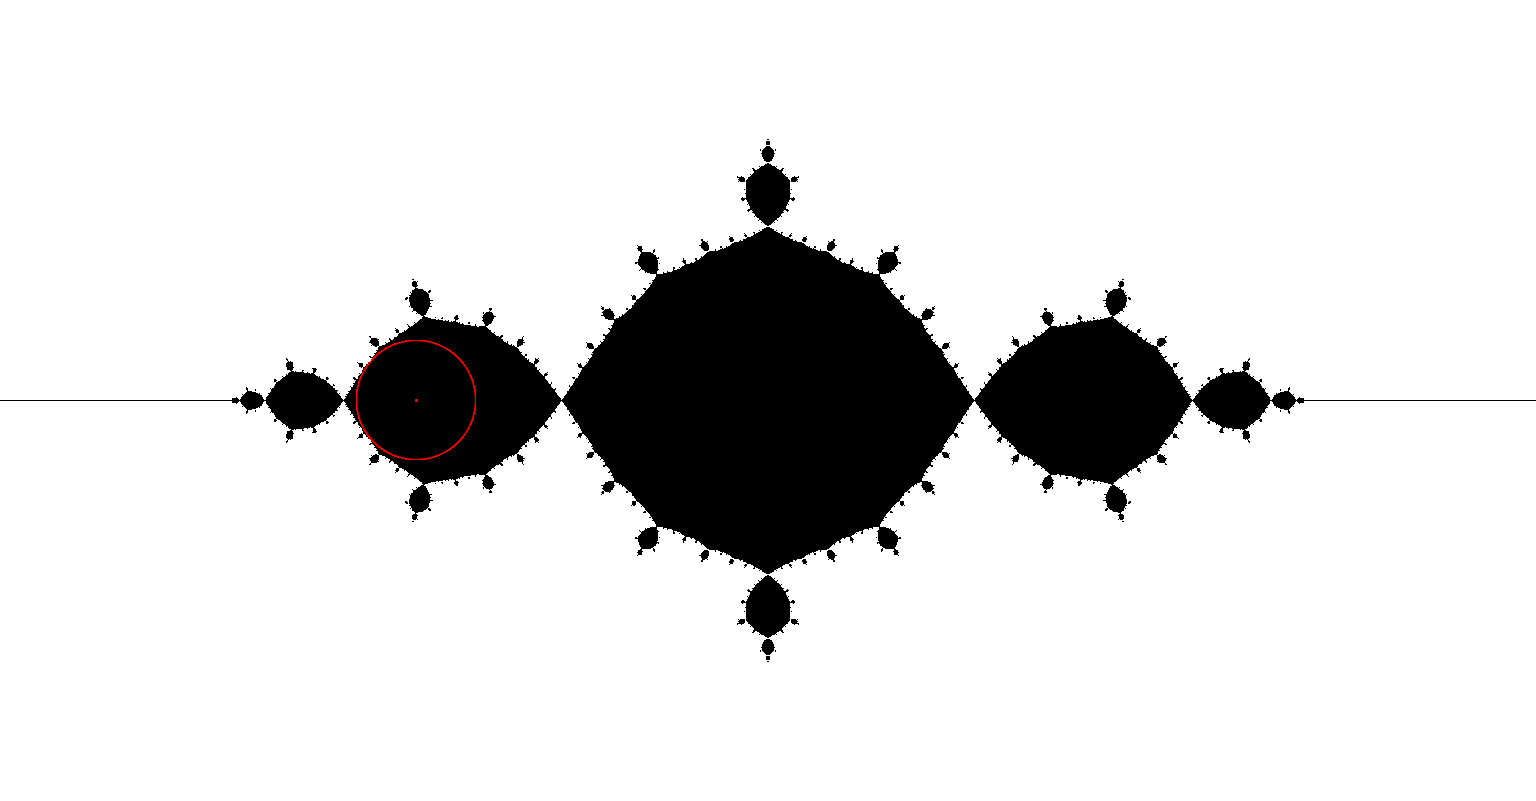
\includegraphics[scale=0.3]{20231028105914}
\textit{$Bas(0)$ (black) for $z \mapsto z^2-1$ with biggest neighbourhood of $w = -1$ that is still in $Bas(0)$ (red).} \\
Image obtained using "Inverted lightness RGB" colourmap of my \textcolor{blue}{\underline{\href{https://github.com/ChrisMzz/pyogl-shader-tester/blob/main/shaders/frag_incriter.glsl}{Julia set shader}}}, with fixed $c$.
\end{center}


\bibliographystyle{alphaurl.bst}
\bibliography{frctl_refs.bib}

\end{document}